\providecommand{\HomA}{\mathrm{Hom}_{A}}
\providecommand{\HomB}{\mathrm{Hom}_{B}}
\providecommand{\HomC}{\mathrm{Hom}_{C}}
\providecommand{\HomD}{\mathrm{Hom}_{D}}
\providecommand{\HomE}{\mathrm{Hom}_{E}}
\providecommand{\HomP}{\mathrm{Hom}_{P}}

\section{正合方块}\label{sec:exact-squares}

为了引出本节的主要定义，让我们试着通过考察一个我们已经理解的特例，来猜测\trInfinityCosmos{}中逐点右\trExtension{}的\trUniversalProperty{}。若外围的\trInfinityCosmos{}是\trCartesianClosed{}，则图表 $f\colon A\to\mathcal{C}$ 沿函子 $k\colon A\to B$ 的逐点右\trExtension{}意在定义「限制函子
$\mathrm{res}_{k}\colon\mathcal{C}^{B}\to\mathcal{C}^{A}$ 在\trElement{} $f\colon 1\to\mathcal{C}^{A}$ 处的\trRightAdjoint{}」之值，而这个\trRightAdjoint{}可能整体存在，也可能不然。对于沿函子 $!\colon A\to 1$ 的扩张情形，限制函子正是定义 2.3.2 中考察的常值图表函子
$\Delta\colon\mathcal{C}\to\mathcal{C}^{A}$，于是经由定义 2.3.8，我们可以把逐点右\trExtension{}理解为计算 $f$ 的\trLimit{}。下述引理描述了这一\trUniversalProperty{}的转置形式。

\begin{lemma}\label{lem:limit-transpose}
在\trCartesianClosed{}\trInfinityCosmos{}中，下左三角形是一个绝对右提升图表——它定义 $f$ 的极限\trElement{}与极限\trCone——当且仅当转置所得的下中三角形具有如下性质：对任何\trInfinityCategory{} $X$，下右的复合图表是一个右\trExtension{}图表。
\begin{center}
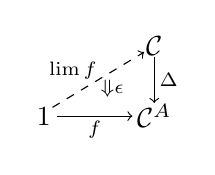
\begin{tikzpicture}[x=1.05em,y=1.05em]
  \node at (0,0) {$1$};
  \node at (3.8,0) {$\mathcal{C}^{A}$};
  \node at (3.8,2.4) {$\mathcal{C}$};
  \draw[->] (0.45,0) -- (3.05,0);
  \node at (1.75,-0.45) {$\scriptstyle f$};
  \draw[->] (3.8,2.05) -- (3.8,0.45);
  \node at (4.3,1.25) {$\scriptstyle\Delta$};
  \draw[->,dashed] (0.3,0.3) -- (3.45,2.2);
  \node at (1.0,1.55) {$\scriptstyle\lim f$};
  \node at (2.35,0.95) {$\scriptstyle\Downarrow\epsilon$};
\end{tikzpicture}
\qquad$\mathrel{\leftrightsquigarrow}$\qquad
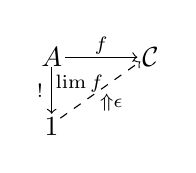
\begin{tikzpicture}[x=1.05em,y=1.05em]
  \node at (0,2.4) {$A$};
  \node at (3.4,2.4) {$\mathcal{C}$};
  \node at (0,0) {$1$};
  \draw[->] (0.45,2.4) -- (2.95,2.4);
  \node at (1.7,2.8) {$\scriptstyle f$};
  \draw[->] (0,2.05) -- (0,0.45);
  \node at (-0.4,1.25) {$\scriptstyle !$};
  \draw[->,dashed] (0.3,0.3) -- (3.05,2.25);
  \node at (0.95,1.5) {$\scriptstyle\lim f$};
  \node at (2.05,0.85) {$\scriptstyle\Uparrow\epsilon$};
\end{tikzpicture}
\qquad
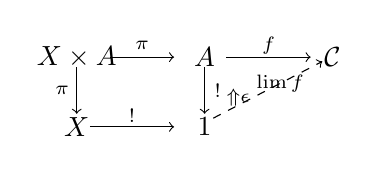
\begin{tikzpicture}[x=1.05em,y=1.05em]
  \node at (0,2.4) {$X\times A$};
  \node at (4.4,2.4) {$A$};
  \node at (8.8,2.4) {$\mathcal{C}$};
  \node at (0,0) {$X$};
  \node at (4.4,0) {$1$};
  \draw[->] (1.15,2.4) -- (3.35,2.4);
  \node at (2.25,2.8) {$\scriptstyle\pi$};
  \draw[->] (5.15,2.4) -- (8.05,2.4);
  \node at (6.6,2.8) {$\scriptstyle f$};
  \draw[->] (0,2.05) -- (0,0.45);
  \node at (-0.5,1.25) {$\scriptstyle\pi$};
  \node at (0.85,1.9) {$\scriptstyle\lrcorner$};
  \draw[->] (4.4,2.05) -- (4.4,0.45);
  \node at (4.85,1.25) {$\scriptstyle !$};
  \draw[->] (0.45,0) -- (3.35,0);
  \node at (1.9,0.38) {$\scriptstyle !$};
  \draw[->,dashed] (4.7,0.3) -- (8.45,2.25);
  \node at (7.0,1.5) {$\scriptstyle\lim f$};
  \node at (5.55,1.0) {$\scriptstyle\Uparrow\epsilon$};
\end{tikzpicture}
\end{center}
\end{lemma}

\begin{proof}
顶点为 $X$ 的一个\trCone{}经由 $f$ 沿常值图表函子的绝对右提升所得的因子分解
\begin{center}
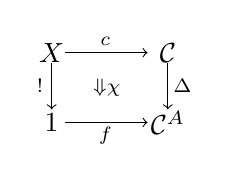
\begin{tikzpicture}[x=1.05em,y=1.05em]
  \node at (0,2.4) {$X$};
  \node at (4.0,2.4) {$\mathcal{C}$};
  \node at (0,0) {$1$};
  \node at (4.0,0) {$\mathcal{C}^{A}$};
  \draw[->] (0.45,2.4) -- (3.3,2.4);
  \node at (1.85,2.8) {$\scriptstyle c$};
  \draw[->] (0,2.05) -- (0,0.45);
  \node at (-0.4,1.25) {$\scriptstyle !$};
  \draw[->] (0.45,0) -- (3.3,0);
  \node at (1.85,-0.45) {$\scriptstyle f$};
  \draw[->] (4.0,2.05) -- (4.0,0.45);
  \node at (4.5,1.25) {$\scriptstyle\Delta$};
  \node at (1.9,1.2) {$\scriptstyle\Downarrow\chi$};
\end{tikzpicture}
\qquad$=$\qquad
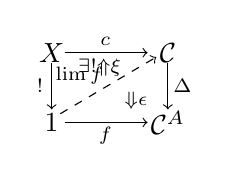
\begin{tikzpicture}[x=1.05em,y=1.05em]
  \node at (0,2.4) {$X$};
  \node at (4.0,2.4) {$\mathcal{C}$};
  \node at (0,0) {$1$};
  \node at (4.0,0) {$\mathcal{C}^{A}$};
  \draw[->] (0.45,2.4) -- (3.3,2.4);
  \node at (1.85,2.8) {$\scriptstyle c$};
  \draw[->] (0,2.05) -- (0,0.45);
  \node at (-0.4,1.25) {$\scriptstyle !$};
  \draw[->] (0.45,0) -- (3.3,0);
  \node at (1.85,-0.45) {$\scriptstyle f$};
  \draw[->] (4.0,2.05) -- (4.0,0.45);
  \node at (4.5,1.25) {$\scriptstyle\Delta$};
  \draw[->,dashed] (0.3,0.3) -- (3.6,2.25);
  \node at (0.95,1.6) {$\scriptstyle\lim f$};
  \node at (2.9,0.75) {$\scriptstyle\Downarrow\epsilon$};
  \node at (1.65,1.9) {$\scriptstyle\exists!\Uparrow\xi$};
\end{tikzpicture}
\end{center}
转置为如下因子分解：
\begin{center}
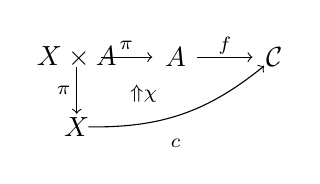
\begin{tikzpicture}[x=1.05em,y=1.05em]
  \node at (0,2.4) {$X\times A$};
  \node at (3.4,2.4) {$A$};
  \node at (6.8,2.4) {$\mathcal{C}$};
  \node at (0,0) {$X$};
  \draw[->] (0.85,2.4) -- (2.6,2.4);
  \node at (1.7,2.8) {$\scriptstyle\pi$};
  \draw[->] (4.15,2.4) -- (6.05,2.4);
  \node at (5.1,2.8) {$\scriptstyle f$};
  \draw[->] (0,2.05) -- (0,0.45);
  \node at (-0.45,1.25) {$\scriptstyle\pi$};
  \draw[->] (0.4,0) to[bend right=20] (6.45,2.1);
  \node at (3.4,-0.55) {$\scriptstyle c$};
  \node at (2.3,1.15) {$\scriptstyle\Uparrow\chi$};
\end{tikzpicture}
\qquad$=$\qquad
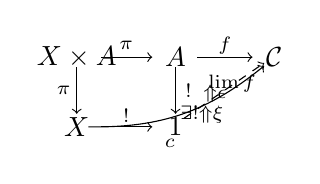
\begin{tikzpicture}[x=1.05em,y=1.05em]
  \node at (0,2.4) {$X\times A$};
  \node at (3.4,2.4) {$A$};
  \node at (6.8,2.4) {$\mathcal{C}$};
  \node at (0,0) {$X$};
  \node at (3.4,0) {$1$};
  \draw[->] (0.85,2.4) -- (2.6,2.4);
  \node at (1.7,2.8) {$\scriptstyle\pi$};
  \draw[->] (4.15,2.4) -- (6.05,2.4);
  \node at (5.1,2.8) {$\scriptstyle f$};
  \draw[->] (0,2.05) -- (0,0.45);
  \node at (-0.45,1.25) {$\scriptstyle\pi$};
  \node at (0.85,1.9) {$\scriptstyle\lrcorner$};
  \draw[->] (3.4,2.05) -- (3.4,0.45);
  \node at (3.85,1.25) {$\scriptstyle !$};
  \draw[->] (0.85,0) -- (2.6,0);
  \node at (1.7,0.38) {$\scriptstyle !$};
  \draw[->] (0.4,0) to[bend right=20] (6.45,2.1);
  \node at (3.2,-0.55) {$\scriptstyle c$};
  \draw[->,dashed] (3.7,0.3) -- (6.45,2.2);
  \node at (5.35,1.5) {$\scriptstyle\lim f$};
  \node at (4.75,1.15) {$\scriptstyle\Uparrow\epsilon$};
  \node at (4.3,0.42) {$\scriptstyle\exists!\Uparrow\xi$};
\end{tikzpicture}
\end{center}
\end{proof}

\cref{lem:limit-transpose}表明：要在一个未必\trCartesianClosed{}\trInfinityCosmos{}中定义 $f\colon A\to\mathcal{C}$ 的\trLimit{}，仅作出 $!\colon A\to 1$ 的右\trExtension{}是不够的。用定义 9.3.1 引入的术语来说，我们还须额外要求：该右\trExtension{}图表与如下形状的方块\emph{粘贴之后保持稳定}：
\begin{center}
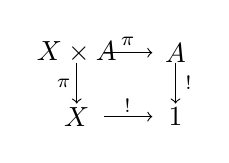
\begin{tikzpicture}[x=1.05em,y=1.05em]
  \node at (0,2.2) {$X\times A$};
  \node at (3.4,2.2) {$A$};
  \node at (0,0) {$X$};
  \node at (3.4,0) {$1$};
  \draw[->] (0.95,2.2) -- (2.6,2.2);
  \node at (1.75,2.6) {$\scriptstyle\pi$};
  \draw[->] (0,1.85) -- (0,0.45);
  \node at (-0.45,1.15) {$\scriptstyle\pi$};
  \node at (0.85,1.7) {$\scriptstyle\lrcorner$};
  \draw[->] (3.4,1.85) -- (3.4,0.45);
  \node at (3.85,1.15) {$\scriptstyle !$};
  \draw[->] (0.95,0) -- (2.6,0);
  \node at (1.75,0.38) {$\scriptstyle !$};
\end{tikzpicture}
\end{center}

我们该如何刻画这样的方块？首先，它们是每条腿都为\trBifibration{}的\trPullback{}。其次，它们是\trCommaSquare，其中\trCommaCone{}是一个恒同 $2$\trCell{}，其指向最好理解为与\cref{lem:limit-transpose}陈述中 $\epsilon$ 相容的方向。\footnote{原书印作「$\nu$」，而引理 9.2.1 全节的 2-胞腔记号为 $\epsilon$，疑为 $\epsilon$ 之误，此处径改。——译者注}由\cref{lem:comma-squares-exact}与\cref{lem:pullback-squares-exact}，我们将看到：这两者都是\emph{\trExactSquare{}}（exact square）的实例，我们现在即引入这一概念。

由命题 8.4.11，\trInfinityCosmos{}的\trHomotopyTwoCategory{}中的\trNaturalTransformation{}与模的\trVirtualEquipment{}中各种形状的一元方块一一对应；特别地，该结果与定理 8.4.4、命题 8.2.4 和命题 8.2.1 一起定义了一个\trCanonical{}双射：
\begin{center}
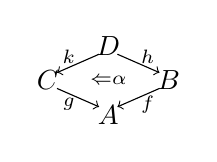
\begin{tikzpicture}[x=0.95em,y=0.95em]
  \node at (0,2.6) {$D$};
  \node at (-2.3,1.3) {$C$};
  \node at (2.3,1.3) {$B$};
  \node at (0,0) {$A$};
  \draw[->] (-0.35,2.3) -- (-1.95,1.6);
  \node at (-1.5,2.2) {$\scriptstyle k$};
  \draw[->] (0.35,2.3) -- (1.95,1.6);
  \node at (1.5,2.2) {$\scriptstyle h$};
  \draw[->] (-1.95,1.0) -- (-0.35,0.3);
  \node at (-1.5,0.4) {$\scriptstyle g$};
  \draw[->] (1.95,1.0) -- (0.35,0.3);
  \node at (1.5,0.4) {$\scriptstyle f$};
  \node at (0,1.3) {$\scriptstyle\Leftarrow\alpha$};
\end{tikzpicture}
\qquad$\mathrel{\leftrightsquigarrow}$\qquad
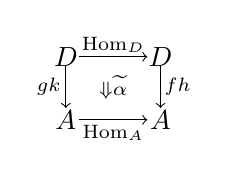
\begin{tikzpicture}[x=0.95em,y=0.95em]
  \node at (0,2.4) {$D$};
  \node at (3.6,2.4) {$D$};
  \node at (0,0) {$A$};
  \node at (3.6,0) {$A$};
  \draw[->] (0.5,2.4) -- (3.1,2.4);
  \node at (1.8,2.85) {$\scriptstyle\HomD$};
  \draw[->] (0.5,0) -- (3.1,0);
  \node at (1.8,-0.5) {$\scriptstyle\HomA$};
  \draw[->] (0,2.05) -- (0,0.45);
  \node at (-0.65,1.25) {$\scriptstyle gk$};
  \draw[->] (3.6,2.05) -- (3.6,0.45);
  \node at (4.25,1.25) {$\scriptstyle fh$};
  \node at (1.8,1.25) {$\scriptstyle\Downarrow\widetilde{\alpha}$};
\end{tikzpicture}
\qquad$\mathrel{\leftrightsquigarrow}$\qquad
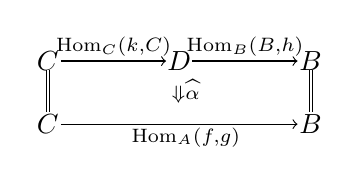
\begin{tikzpicture}[x=0.95em,y=0.95em]
  \node at (0,2.4) {$C$};
  \node at (5.0,2.4) {$D$};
  \node at (10.0,2.4) {$B$};
  \node at (0,0) {$C$};
  \node at (10.0,0) {$B$};
  \draw[->] (0.5,2.4) -- (4.5,2.4);
  \node at (2.5,2.95) {$\scriptstyle\HomC(k,C)$};
  \draw[->] (5.5,2.4) -- (9.5,2.4);
  \node at (7.5,2.95) {$\scriptstyle\HomB(B,h)$};
  \draw[double,double distance=0.6pt] (0,2.05) -- (0,0.45);
  \draw[double,double distance=0.6pt] (10.0,2.05) -- (10.0,0.45);
  \draw[->] (0.5,0) -- (9.5,0);
  \node at (5.25,-0.5) {$\scriptstyle\HomA(f,g)$};
  \node at (5.25,1.25) {$\scriptstyle\Downarrow\widehat{\alpha}$};
\end{tikzpicture}
\end{center}

\begin{definition}[\trExactSquare]\label{def:exact-square}
\trInfinityCosmos{}的\trHomotopyTwoCategory{}中的一个方块
\begin{center}
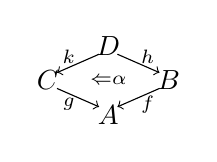
\begin{tikzpicture}[x=0.95em,y=0.95em]
  \node at (0,2.6) {$D$};
  \node at (-2.3,1.3) {$C$};
  \node at (2.3,1.3) {$B$};
  \node at (0,0) {$A$};
  \draw[->] (-0.35,2.3) -- (-1.95,1.6);
  \node at (-1.5,2.2) {$\scriptstyle k$};
  \draw[->] (0.35,2.3) -- (1.95,1.6);
  \node at (1.5,2.2) {$\scriptstyle h$};
  \draw[->] (-1.95,1.0) -- (-0.35,0.3);
  \node at (-1.5,0.4) {$\scriptstyle g$};
  \draw[->] (1.95,1.0) -- (0.35,0.3);
  \node at (1.5,0.4) {$\scriptstyle f$};
  \node at (0,1.3) {$\scriptstyle\Leftarrow\alpha$};
\end{tikzpicture}
\end{center}
是\textbf{正合的}\footnote{遗憾的是，「正合方块」这一术语在各种不同的场合都有使用。我们希望上下文足以表明，此处引入的概念与稳定\trInfinityCategory{}中既是推出又是拉回的方块毫无关系。练习 9.4.ii 揭示了这一正合方块概念与伴随函子之间对应为同构的交换方块二者之间的联系（见命题 6.3.10）。}%
，当且仅当左下所示的对应\trCell{}——它在引理 8.1.16 的双射之下编码为右下所示的粘贴复合
\begin{rveq}\label{eq:exact-square-cell}
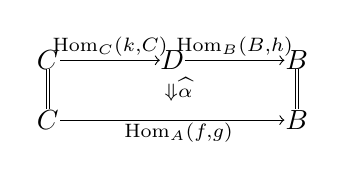
\begin{tikzpicture}[x=0.9em,y=0.9em]
  \node at (0,2.6) {$C$};
  \node at (5.0,2.6) {$D$};
  \node at (10.0,2.6) {$B$};
  \node at (0,0.2) {$C$};
  \node at (10.0,0.2) {$B$};
  \draw[->] (0.5,2.6) -- (4.5,2.6);
  \node at (2.5,3.15) {$\scriptstyle\HomC(k,C)$};
  \draw[->] (5.5,2.6) -- (9.5,2.6);
  \node at (7.5,3.15) {$\scriptstyle\HomB(B,h)$};
  \draw[double,double distance=0.6pt] (0,2.25) -- (0,0.65);
  \draw[double,double distance=0.6pt] (10.0,2.25) -- (10.0,0.65);
  \draw[->] (0.5,0.2) -- (9.5,0.2);
  \node at (5.25,-0.3) {$\scriptstyle\HomA(f,g)$};
  \node at (5.25,1.45) {$\scriptstyle\Downarrow\widehat{\alpha}$};
\end{tikzpicture}
\qquad\mathrel{\leftrightsquigarrow}\qquad
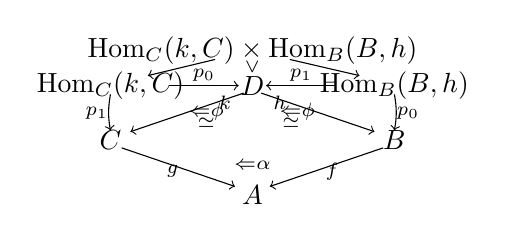
\begin{tikzpicture}[x=0.9em,y=0.9em]
  \node at (2.7,6.0) {$\HomC(k,C)\times\HomB(B,h)$};
  \node at (2.7,5.35) {$\scriptstyle\vee$};
  \draw[->] (1.2,5.65) -- (-1.5,5.0);
  \draw[->] (4.2,5.65) -- (7.0,5.0);
  \node at (-3.0,4.6) {$\HomC(k,C)$};
  \node at (2.7,4.6) {$D$};
  \node at (8.4,4.6) {$\HomB(B,h)$};
  \draw[->] (-0.65,4.6) -- (2.15,4.6);
  \node at (0.75,5.0) {$\scriptstyle p_{0}$};
  \draw[->] (6.05,4.6) -- (3.25,4.6);
  \node at (4.65,5.0) {$\scriptstyle p_{1}$};
  \draw[->] (-3.0,4.25) to[bend right=10] (-3.0,2.8);
  \node at (-3.55,3.5) {$\scriptstyle p_{1}$};
  \draw[->] (8.4,4.25) to[bend left=10] (8.4,2.8);
  \node at (8.95,3.5) {$\scriptstyle p_{0}$};
  \node at (0.85,3.55) {$\scriptstyle\Leftarrow\phi$};
  \node at (0.85,3.1) {$\scriptstyle\simeq$};
  \node at (4.5,3.55) {$\scriptstyle\Leftarrow\phi$};
  \node at (4.25,3.1) {$\scriptstyle\simeq$};
  \draw[->] (2.35,4.3) -- (-2.2,2.75);
  \node at (1.6,3.9) {$\scriptstyle k$};
  \draw[->] (3.05,4.3) -- (7.6,2.75);
  \node at (3.8,3.9) {$\scriptstyle h$};
  \node at (-3.0,2.4) {$C$};
  \node at (8.4,2.4) {$B$};
  \node at (2.7,0.2) {$A$};
  \draw[->] (-2.55,2.1) -- (2.0,0.55);
  \node at (-0.5,1.15) {$\scriptstyle g$};
  \draw[->] (7.95,2.1) -- (3.4,0.55);
  \node at (5.9,1.15) {$\scriptstyle f$};
  \node at (2.7,1.4) {$\scriptstyle\Leftarrow\alpha$};
\end{tikzpicture}
\end{rveq}
{\emergencystretch=6em
——把 $\HomA(f,g)$ 显示为定义 8.3.1 所定义意义下的复合
$\HomC(k,C)\otimes\HomB(B,h)$。\par}
\end{definition}

当边界方块在上下文中自明时，为节省语言，我们可以写「$\alpha\colon fh\Rightarrow gk$ 是一个正合方块」；但需注意，若被 $2$\trCell{} $\alpha$ 所栖居的方块的四条边界箭头中任何一条的位置发生移动，正合性条件的含义便会随之改变。\footnote{例如，比较\cref{lem:trivial-exact-squares}与引理 9.4.4 的陈述。}%

\begin{remark}[作为 Beck--Chevalley 条件的正合性]\label{rem:beck-chevalley}
由推论 8.4.8，由\trOneCellInduction{}所定义的如下\trSpan{}映射
\begin{center}
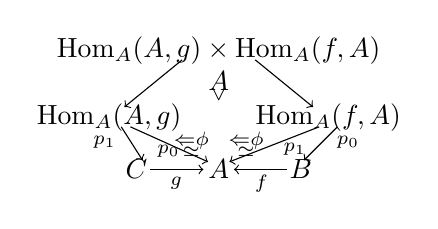
\begin{tikzpicture}[x=1.1em,y=1.1em]
  \node at (2.7,4.8) {$\HomA(A,g)\times\HomA(f,A)$};
  \node at (2.7,3.8) {$A$};
  \node at (2.7,3.35) {$\scriptstyle\vee$};
  \draw[->] (1.5,4.5) -- (-0.4,2.95);
  \draw[->] (3.9,4.5) -- (5.8,2.95);
  \node at (-0.9,2.6) {$\HomA(A,g)$};
  \node at (6.3,2.6) {$\HomA(f,A)$};
  \draw[->] (-0.5,2.3) -- (0.2,1.2);
  \node at (-1.05,1.8) {$\scriptstyle p_{1}$};
  \draw[->] (-0.2,2.3) -- (2.35,1.15);
  \node at (1.05,1.5) {$\scriptstyle p_{0}$};
  \draw[->] (6.0,2.3) -- (3.05,1.15);
  \node at (5.2,1.55) {$\scriptstyle p_{1}$};
  \draw[->] (6.6,2.3) -- (5.5,1.2);
  \node at (6.95,1.8) {$\scriptstyle p_{0}$};
  \node at (1.8,1.85) {$\scriptstyle\Leftarrow\phi$};
  \node at (1.8,1.47) {$\scriptstyle\simeq$};
  \node at (3.6,1.85) {$\scriptstyle\Leftarrow\phi$};
  \node at (3.6,1.47) {$\scriptstyle\simeq$};
  \node at (0,0.9) {$C$};
  \node at (2.7,0.9) {$A$};
  \node at (5.4,0.9) {$B$};
  \draw[->] (0.45,0.9) -- (2.2,0.9);
  \node at (1.3,0.45) {$\scriptstyle g$};
  \draw[->] (4.95,0.9) -- (3.2,0.9);
  \node at (4.1,0.45) {$\scriptstyle f$};
\end{tikzpicture}
\qquad$=$\qquad
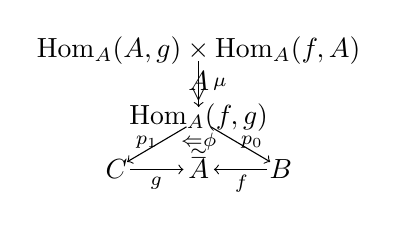
\begin{tikzpicture}[x=1.1em,y=1.1em]
  \node at (2.7,4.8) {$\HomA(A,g)\times\HomA(f,A)$};
  \node at (2.7,3.8) {$A$};
  \node at (2.7,3.35) {$\scriptstyle\vee$};
  \draw[->] (2.7,4.45) -- (2.7,2.95);
  \node at (3.4,3.7) {$\scriptstyle\ulcorner\mu\urcorner$};
  \node at (2.7,2.6) {$\HomA(f,g)$};
  \draw[->] (2.3,2.3) -- (0.35,1.15);
  \node at (1.0,1.8) {$\scriptstyle p_{1}$};
  \draw[->] (3.1,2.3) -- (5.05,1.15);
  \node at (4.45,1.8) {$\scriptstyle p_{0}$};
  \node at (2.7,1.8) {$\scriptstyle\Leftarrow\phi$};
  \node at (2.7,1.42) {$\scriptstyle\simeq$};
  \node at (0,0.9) {$C$};
  \node at (2.7,0.9) {$A$};
  \node at (5.4,0.9) {$B$};
  \draw[->] (0.45,0.9) -- (2.2,0.9);
  \node at (1.3,0.45) {$\scriptstyle g$};
  \draw[->] (4.95,0.9) -- (3.2,0.9);
  \node at (4.1,0.45) {$\scriptstyle f$};
\end{tikzpicture}
\end{center}
编码了一个二元\trCell{}
$\mu\colon\HomA(A,g)\divideontimes\HomA(f,A)\Rightarrow\HomA(f,g)$，它是一个复合。正合性说，$\alpha$ 诱导了从 $C$ 到 $B$ 的模的如下\trIsomorphism
\begin{equation*}
\widehat{\alpha}\colon\HomC(k,C)\otimes\HomB(B,h)\simeq\HomA(A,g)\otimes\HomA(f,A)
\end{equation*}
\end{remark}

\begin{digression}[强正合性]\label{dig:strong-exactness}
回忆 8.3 节：在任何\trVirtualEquipment{}中出现的许多形式地定义的复合\trCell{}，在与一个\trInfinityCosmos{}相联系的模的\trVirtualEquipment{}中实际上是强复合。基于这一经验，人们或许会预期：我们在模的\trVirtualEquipment{}中遇到的许多\trExactSquare{}实际上都是\textbf{强正合}的，意即\trCell{}
$\widehat{\alpha}\colon\HomC(k,C)\divideontimes\HomB(B,h)\Rightarrow\HomA(f,g)$ 是一个强复合——而事实也确实如此。事实上，在 $(\infty,1)$-范畴的\trInfinityCosmos{}中，所有复合都存在且都是强的：模的张量积可以通过一种对\trPullback{}稳定的逐纤维的余反转器（coinverter）构造来定义。由于模的任何相容序列的复合都等价于强复合，在这类\trInfinityCosmos{}中，所有复合、从而所有\trExactSquare{}都自动满足更强的\trUniversalProperty{}。

\trExactSquare{}在此处扮演的主要角色，是发展逐点左\trExtension{}与右\trExtension{}的概念；为此，较弱的 2-范畴性\trUniversalProperty{}已然足够。我们顺带指出：我们形式地定义的\trExactSquare{}都是强的，但在证明中我们通常只诉诸较弱的正合性质。仅有一种情形下更强的正合性概念可能更为妥当，我们将在注 9.4.12 中讨论它。
\end{digression}

本节的其余部分致力于\trExactSquare{}的例子。

\begin{lemma}[\trCommaSquare{}是正合的]\label{lem:comma-squares-exact}
对任何余跨度 $C\overset{g}{\to}A\overset{f}{\gets}B$，\trCommaCone{}定义了一个强正合方块：
\begin{center}
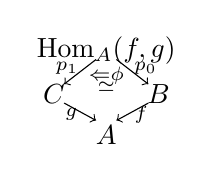
\begin{tikzpicture}[x=1.05em,y=1.05em]
  \node at (0,2.4) {$\HomA(f,g)$};
  \draw[->] (-0.35,2.1) -- (-1.45,1.25);
  \node at (-1.35,1.8) {$\scriptstyle p_{1}$};
  \draw[->] (0.35,2.1) -- (1.45,1.25);
  \node at (1.35,1.8) {$\scriptstyle p_{0}$};
  \node at (-1.8,0.9) {$C$};
  \node at (1.8,0.9) {$B$};
  \node at (0,1.55) {$\scriptstyle\Leftarrow\phi$};
  \node at (0,1.15) {$\scriptstyle\simeq$};
  \draw[->] (-1.45,0.6) -- (-0.35,0.0);
  \node at (-1.2,0.2) {$\scriptstyle g$};
  \draw[->] (1.45,0.6) -- (0.35,0.0);
  \node at (1.2,0.2) {$\scriptstyle f$};
  \node at (0,-0.5) {$A$};
\end{tikzpicture}
\end{center}
\end{lemma}

\begin{proof}
由命题 8.3.11，模 $C\xrightarrow{\HomA(f,g)}B$ 是其左腿的左表示后接其右腿的右表示而成的强复合。由注 8.3.13，二元复合\trCell{}
$\HomC(p_{1},C)\divideontimes\HomB(B,p_{0})\Rightarrow\HomA(f,g)$ 在引理 8.1.16 的双射之下对应于粘贴复合
\begin{center}
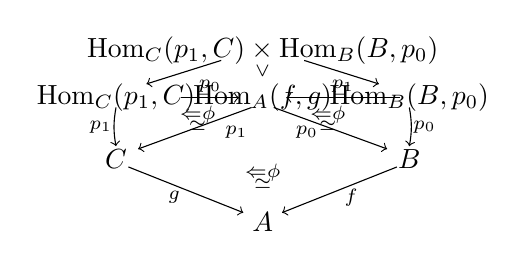
\begin{tikzpicture}[x=1.0em,y=1.0em]
  \node at (2.7,5.9) {$\HomC(p_{1},C)\times\HomB(B,p_{0})$};
  \node at (2.7,5.15) {$\scriptstyle\vee$};
  \draw[->] (1.2,5.55) -- (-1.5,4.7);
  \draw[->] (4.2,5.55) -- (6.9,4.7);
  \node at (-2.6,4.2) {$\HomC(p_{1},C)$};
  \node at (2.7,4.2) {$\HomA(f,g)$};
  \node at (8.0,4.2) {$\HomB(B,p_{0})$};
  \draw[->] (-0.25,4.2) -- (1.85,4.2);
  \node at (0.8,4.62) {$\scriptstyle p_{0}$};
  \draw[->] (7.65,4.2) -- (3.55,4.2);
  \node at (5.6,4.62) {$\scriptstyle p_{1}$};
  \draw[->] (-2.6,3.85) to[bend right=10] (-2.6,2.45);
  \node at (-3.15,3.15) {$\scriptstyle p_{1}$};
  \draw[->] (8.0,3.85) to[bend left=10] (8.0,2.45);
  \node at (8.55,3.15) {$\scriptstyle p_{0}$};
  \node at (0.35,3.6) {$\scriptstyle\Leftarrow\phi$};
  \node at (0.35,3.2) {$\scriptstyle\simeq$};
  \node at (5.05,3.6) {$\scriptstyle\Leftarrow\phi$};
  \node at (5.05,3.2) {$\scriptstyle\simeq$};
  \draw[->] (2.3,3.85) -- (-1.8,2.35);
  \node at (1.75,2.95) {$\scriptstyle p_{1}$};
  \draw[->] (3.1,3.85) -- (7.2,2.35);
  \node at (4.3,2.95) {$\scriptstyle p_{0}$};
  \node at (-2.6,2.0) {$C$};
  \node at (8.0,2.0) {$B$};
  \node at (2.7,1.5) {$\scriptstyle\Leftarrow\phi$};
  \node at (2.7,1.1) {$\scriptstyle\simeq$};
  \draw[->] (-2.15,1.7) -- (2.0,0.05);
  \node at (-0.5,0.6) {$\scriptstyle g$};
  \draw[->] (7.55,1.7) -- (3.4,0.05);
  \node at (5.9,0.6) {$\scriptstyle f$};
  \node at (2.7,-0.3) {$A$};
\end{tikzpicture}
\end{center}
这便恢复了由 \eqref{eq:exact-square-cell} 所定义的、检验\trCommaSquare
$\phi\colon fp_{0}\Rightarrow gp_{1}$ 正合性的胞腔 $\widehat{\phi}$。
\end{proof}

\begin{lemma}\label{lem:pullback-squares-exact}
若 $g\colon C\to A$ 是一个\trCartesianFibration{}或 $f\colon B\to A$ 是一个\trCocartesianFibration{}，则此\trPullback{}方块是强正合的：
\begin{center}
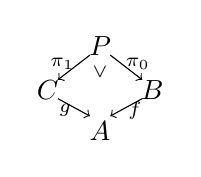
\begin{tikzpicture}[x=1.05em,y=1.05em]
  \node at (0,2.4) {$P$};
  \draw[->] (-0.35,2.1) -- (-1.45,1.25);
  \node at (-1.3,1.8) {$\scriptstyle\pi_{1}$};
  \node at (0,1.5) {$\scriptstyle\vee$};
  \draw[->] (0.35,2.1) -- (1.45,1.25);
  \node at (1.3,1.8) {$\scriptstyle\pi_{0}$};
  \node at (-1.8,0.9) {$C$};
  \node at (1.8,0.9) {$B$};
  \draw[->] (-1.45,0.6) -- (-0.35,0.0);
  \node at (-1.2,0.2) {$\scriptstyle g$};
  \draw[->] (1.45,0.6) -- (0.35,0.0);
  \node at (1.2,0.2) {$\scriptstyle f$};
  \node at (0,-0.5) {$A$};
\end{tikzpicture}
\end{center}
\end{lemma}

\begin{proof}
这两个断言是对偶的，不过——正如证明所揭示的——余笛卡尔纤维化与笛卡尔纤维化的位置不可互换。若 $f\colon B\to A$ 是一个\trCocartesianFibration{}，注意到：由恒同 $2$\trCell{} $f\pi_{0}=g\pi_{1}$ 诱导的函子 $\Delta\colon P\to\HomA(f,g)$，是由恒同 $2$\trCell{} $\mathrm{id}_{f}$ 诱导的函子 $\Delta_{f}\colon B\to\HomA(f,A)$ 的一个\trPullback{}：
\begin{center}
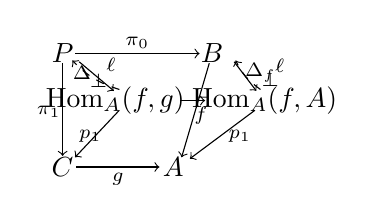
\begin{tikzpicture}[x=1.0em,y=1.0em]
  \node at (0,3.2) {$P$};
  \node at (5.4,3.2) {$B$};
  \draw[->] (0.45,3.2) -- (4.95,3.2);
  \node at (2.7,3.6) {$\scriptstyle\pi_{0}$};
  \draw[->] (0.6,2.9) -- (1.85,1.85);
  \node at (0.7,2.5) {$\scriptstyle\Delta$};
  \draw[->,dashed] (2.05,1.9) to[bend left=14] (0.35,2.95);
  \node at (1.75,2.8) {$\scriptstyle\ell$};
  \node at (1.3,2.2) {$\scriptstyle\perp$};
  \draw[->] (6.2,2.9) -- (7.0,1.85);
  \node at (7.15,2.5) {$\scriptstyle\Delta_{f}$};
  \draw[->,dashed] (7.15,1.9) to[bend left=14] (6.25,2.95);
  \node at (7.85,2.75) {$\scriptstyle\ell$};
  \node at (7.5,2.25) {$\scriptstyle\perp$};
  \node at (1.9,1.5) {$\HomA(f,g)$};
  \node at (7.3,1.5) {$\HomA(f,A)$};
  \draw[->] (4.25,1.5) -- (5.15,1.5);
  \node at (1.9,1.0) {$\scriptstyle\lrcorner$};
  \draw[->] (0,2.85) -- (0,-0.5);
  \node at (-0.5,1.1) {$\scriptstyle\pi_{1}$};
  \draw[->] (2.05,1.15) -- (0.45,-0.55);
  \node at (1.0,0.2) {$\scriptstyle p_{1}$};
  \draw[->] (5.3,2.85) -- (4.3,-0.55);
  \node at (5.0,0.95) {$\scriptstyle f$};
  \draw[->] (6.95,1.15) -- (4.6,-0.6);
  \node at (6.4,0.2) {$\scriptstyle p_{1}$};
  \node at (0,-0.9) {$C$};
  \node at (4.0,-0.9) {$A$};
  \draw[->] (0.5,-0.9) -- (3.5,-0.9);
  \node at (2.0,-1.35) {$\scriptstyle g$};
\end{tikzpicture}
\end{center}
由于 $f$ 是\trCocartesianFibration{}，定理 5.2.8(iii) 告诉我们：$\Delta_{f}\colon B\to\HomA(f,A)$ 在 $A$ 上带有一个\trFiberedAdjunction{}。这一\trFiberedAdjunction{}沿 $g\colon C\to A$ 作\trPullback{}之后，便给出 $\Delta\colon P\to\HomA(f,g)$ 的一个\trFiberedAdjunction{}。
由于 $\pi_{0}=p_{0}\Delta$，推论 8.4.9 蕴含：\trCanonical{}\trCell
\begin{equation*}
\begin{aligned}
&\mathrm{Hom}^{\HomA(f,g)}(\HomA(f,g),\Delta)\\
&\divideontimes\HomB(B,p_{0})\Rightarrow\HomB(B,\pi_{0})
\end{aligned}
\end{equation*}
{\emergencystretch=6em
是一个强复合。由于 $\ell\dashv\Delta$，由命题 4.1.1 存在\trEquivalence{}
$\HomP(\ell,P)\simeq\allowbreak\mathrm{Hom}_{\HomA(f,g)}(\HomA(f,g),\Delta)$。又由于 $p_{1}=\pi_{1}\ell$，由推论 8.4.9，\trCanonical{}\trCell
\begin{equation*}
\HomC(\pi_{1},C)\divideontimes\HomP(\ell,P)\Rightarrow\HomC(p_{1},C)
\end{equation*}}
是一个强复合。将这些双射复合起来，我们便看到：定义域为
$\HomC(\pi_{1},C)\divideontimes\HomB(B,\pi_{0})$ 的\trCell{}与定义域为
$\HomC(p_{1},C)\divideontimes\HomB(B,p_{0})$ 的\trCell{}之间一一对应。
由于 $\ell\dashv\Delta$ 是一个\trFiberedAdjunction{}，\trNaturalTransformation{}
$\phi\colon fp_{0}\Rightarrow gp_{1}=g\pi_{1}\ell$ 沿 $\ell\dashv\Delta$ 的转置等于
$\phi\Delta=\mathrm{id}\colon f\pi_{0}=fp_{0}i\Rightarrow gp_{1}i=g\pi_{1}$。这说明，如下两\trCell
\begin{equation*}
\begin{aligned}
\widehat{\mathrm{id}}&\colon\HomC(\pi_{1},C)\divideontimes\HomB(B,\pi_{0})\Rightarrow\HomA(f,g),\\
\widehat{\phi}&\colon\HomC(p_{1},C)\divideontimes\HomB(B,p_{0})\Rightarrow\HomA(f,g)
\end{aligned}
\end{equation*}
在刚刚描述的双射之下相互对应。由于\cref{lem:comma-squares-exact}证明了 $\widehat{\phi}$ 是一个强复合，由引理 8.3.8，$\widehat{\mathrm{id}}$ 亦然。
\end{proof}

为了后续使用，我们在此记录\trExactSquare{}的一些平凡例子。

\begin{lemma}\label{lem:trivial-exact-squares}
对任何一对函子 $k\colon A\to B$ 与 $h\colon C\to D$，\trPullback{}方块是强正合的：
\begin{center}
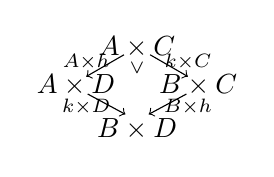
\begin{tikzpicture}[x=1.05em,y=1.05em]
  \node at (0,2.4) {$A\times C$};
  \draw[->] (-0.45,2.15) -- (-1.75,1.4);
  \node at (-1.75,1.9) {$\scriptstyle A\times h$};
  \node at (0,1.7) {$\scriptstyle\vee$};
  \draw[->] (0.45,2.15) -- (1.75,1.4);
  \node at (1.75,1.9) {$\scriptstyle k\times C$};
  \node at (-2.1,1.1) {$A\times D$};
  \node at (2.1,1.1) {$B\times C$};
  \draw[->] (-1.7,0.8) -- (-0.4,0.1);
  \node at (-1.75,0.35) {$\scriptstyle k\times D$};
  \draw[->] (1.7,0.8) -- (0.4,0.1);
  \node at (1.75,0.35) {$\scriptstyle B\times h$};
  \node at (0,-0.4) {$B\times D$};
\end{tikzpicture}
\end{center}
特别地，恒同\trCell{}定义强正合方块：
\begin{center}
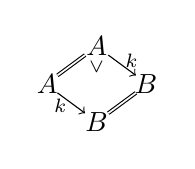
\begin{tikzpicture}[x=1.05em,y=1.05em]
  \node at (0,2.4) {$A$};
  \draw[double,double distance=0.6pt] (-0.4,2.1) -- (-1.35,1.4);
  \node at (0,1.7) {$\scriptstyle\vee$};
  \draw[->] (0.4,2.1) -- (1.35,1.4);
  \node at (1.2,1.9) {$\scriptstyle k$};
  \node at (-1.7,1.1) {$A$};
  \node at (1.7,1.1) {$B$};
  \draw[->] (-1.35,0.8) -- (-0.4,0.1);
  \node at (-1.25,0.35) {$\scriptstyle k$};
  \draw[double,double distance=0.6pt] (1.35,0.8) -- (0.4,0.1);
  \node at (0,-0.2) {$B$};
\end{tikzpicture}
\qquad
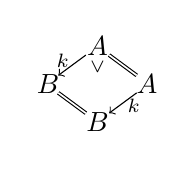
\begin{tikzpicture}[x=1.05em,y=1.05em]
  \node at (0,2.4) {$A$};
  \draw[->] (-0.4,2.1) -- (-1.35,1.4);
  \node at (-1.2,1.9) {$\scriptstyle k$};
  \node at (0,1.7) {$\scriptstyle\vee$};
  \draw[double,double distance=0.6pt] (0.4,2.1) -- (1.35,1.4);
  \node at (-1.7,1.1) {$B$};
  \node at (1.7,1.1) {$A$};
  \draw[double,double distance=0.6pt] (-1.35,0.8) -- (-0.4,0.1);
  \draw[->] (1.35,0.8) -- (0.4,0.1);
  \node at (1.25,0.35) {$\scriptstyle k$};
  \node at (0,-0.2) {$B$};
\end{tikzpicture}
\end{center}
\end{lemma}

\begin{proof}
\cref{ex:prove-trivial-exact-squares}。
\end{proof}

最后，刚刚建立的这些\trExactSquare{}还可以复合起来，产生进一步的\trExactSquare{}：

\begin{lemma}[正合方块的复合]\label{lem:composites-exact-squares}
给定\trHomotopyTwoCategory{}中如下图式所示的方块图表
\begin{center}
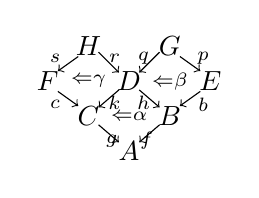
\begin{tikzpicture}[x=1.05em,y=1.05em]
  \node at (-1.4,2.9) {$H$};
  \node at (1.4,2.9) {$G$};
  \node at (-2.8,1.7) {$F$};
  \node at (0,1.7) {$D$};
  \node at (2.8,1.7) {$E$};
  \node at (-1.4,0.5) {$C$};
  \node at (1.4,0.5) {$B$};
  \node at (0,-0.7) {$A$};
  \draw[->] (-1.75,2.55) -- (-2.45,2.05);
  \node at (-2.55,2.5) {$\scriptstyle s$};
  \draw[->] (-1.05,2.7) -- (-0.35,2.0);
  \node at (-0.5,2.5) {$\scriptstyle r$};
  \draw[->] (1.05,2.7) -- (0.35,2.0);
  \node at (0.5,2.5) {$\scriptstyle q$};
  \draw[->] (1.75,2.55) -- (2.45,2.05);
  \node at (2.55,2.5) {$\scriptstyle p$};
  \draw[->] (-2.45,1.35) -- (-1.75,0.85);
  \node at (-2.55,0.9) {$\scriptstyle c$};
  \draw[->] (-0.35,1.4) -- (-1.05,0.8);
  \node at (-0.5,0.95) {$\scriptstyle k$};
  \draw[->] (0.35,1.4) -- (1.05,0.8);
  \node at (0.5,0.95) {$\scriptstyle h$};
  \draw[->] (2.45,1.35) -- (1.75,0.85);
  \node at (2.55,0.9) {$\scriptstyle b$};
  \draw[->] (-1.05,0.2) -- (-0.35,-0.4);
  \node at (-0.6,-0.35) {$\scriptstyle g$};
  \draw[->] (1.05,0.2) -- (0.35,-0.4);
  \node at (0.6,-0.35) {$\scriptstyle f$};
  \node at (-1.4,1.7) {$\scriptstyle\Leftarrow\gamma$};
  \node at (1.4,1.7) {$\scriptstyle\Leftarrow\beta$};
  \node at (0,0.5) {$\scriptstyle\Leftarrow\alpha$};
\end{tikzpicture}
\end{center}
若 $\alpha\colon fh\Rightarrow gk$、$\beta\colon bp\Rightarrow hq$ 与
$\gamma\colon kr\Rightarrow cs$ 都是正合方块，则复合矩形
$\alpha q\cdot f\beta$ 与 $g\gamma\cdot\alpha r$ 也是正合方块；且当构成它们的方块都强正合时，这两个矩形也强正合。由此，（强）正合方块的任意「\trDoubleCategory{}式」复合都定义（强）正合方块。
\end{lemma}

\begin{proof}
这两种情形互为余对偶，故只需证明矩形
$\alpha q\cdot f\beta\colon g(kq)\Rightarrow(fb)p$ 是正合的。对应的胞腔
$\widehat{\alpha q\cdot f\beta}$ 显示于下左，它经由复合 $\widehat{\beta}$ 在下右分解：
\begin{center}
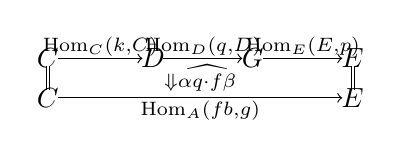
\begin{tikzpicture}[x=0.95em,y=0.95em]
  \node at (-4.6,1.2) {$C$};
  \node at (-0.6,1.2) {$D$};
  \node at (3.2,1.2) {$G$};
  \node at (7.0,1.2) {$E$};
  \draw[->] (-4.2,1.2) -- (-1.0,1.2);
  \node at (-2.6,1.65) {$\scriptstyle\HomC(k,C)$};
  \draw[->] (-0.2,1.2) -- (2.8,1.2);
  \node at (1.3,1.65) {$\scriptstyle\HomD(q,D)$};
  \draw[->] (3.6,1.2) -- (6.6,1.2);
  \node at (5.1,1.65) {$\scriptstyle\HomE(E,p)$};
  \draw[double,double distance=0.6pt] (-4.6,0.9) -- (-4.6,0.0);
  \draw[double,double distance=0.6pt] (7.0,0.9) -- (7.0,0.0);
  \node at (1.2,0.45) {$\scriptstyle\Downarrow\widehat{\alpha q\cdot f\beta}$};
  \node at (-4.6,-0.3) {$C$};
  \node at (7.0,-0.3) {$E$};
  \draw[->] (-4.2,-0.3) -- (6.6,-0.3);
  \node at (1.2,-0.8) {$\scriptstyle\HomA(fb,g)$};
\end{tikzpicture}
\qquad$=$\qquad
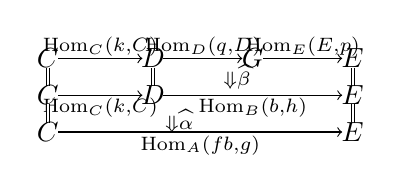
\begin{tikzpicture}[x=0.95em,y=0.95em]
  \node at (-4.6,2.3) {$C$};
  \node at (-0.6,2.3) {$D$};
  \node at (3.2,2.3) {$G$};
  \node at (7.0,2.3) {$E$};
  \draw[->] (-4.2,2.3) -- (-1.0,2.3);
  \node at (-2.6,2.75) {$\scriptstyle\HomC(k,C)$};
  \draw[->] (-0.2,2.3) -- (2.8,2.3);
  \node at (1.3,2.75) {$\scriptstyle\HomD(q,D)$};
  \draw[->] (3.6,2.3) -- (6.6,2.3);
  \node at (5.1,2.75) {$\scriptstyle\HomE(E,p)$};
  \draw[double,double distance=0.6pt] (-4.6,1.95) -- (-4.6,1.25);
  \draw[double,double distance=0.6pt] (-0.6,1.95) -- (-0.6,1.25);
  \draw[double,double distance=0.6pt] (7.0,1.95) -- (7.0,1.25);
  \node at (2.6,1.6) {$\scriptstyle\Downarrow\widehat{\beta}$};
  \node at (-4.6,0.9) {$C$};
  \node at (-0.6,0.9) {$D$};
  \node at (7.0,0.9) {$E$};
  \draw[->] (-4.2,0.9) -- (-1.0,0.9);
  \node at (-2.6,0.42) {$\scriptstyle\HomC(k,C)$};
  \draw[->] (-0.2,0.9) -- (6.6,0.9);
  \node at (3.2,0.42) {$\scriptstyle\HomB(b,h)$};
  \draw[double,double distance=0.6pt] (-4.6,0.55) -- (-4.6,-0.15);
  \draw[double,double distance=0.6pt] (7.0,0.55) -- (7.0,-0.15);
  \node at (0.4,-0.1) {$\scriptstyle\Downarrow\widehat{\alpha}$};
  \node at (-4.6,-0.5) {$C$};
  \node at (7.0,-0.5) {$E$};
  \draw[->] (-4.2,-0.5) -- (6.6,-0.5);
  \node at (1.2,-1.0) {$\scriptstyle\HomA(fb,g)$};
\end{tikzpicture}
\end{center}
而将 \eqref{eq:exact-square-cell} 中的公式与引理 8.1.16 相比较，我们看到胞腔
$\widehat{\alpha}$ 满足如下粘贴等式：
\begin{center}
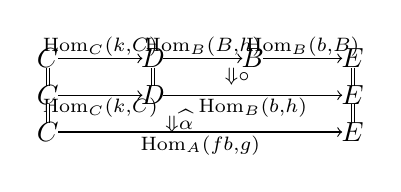
\begin{tikzpicture}[x=0.95em,y=0.95em]
  \node at (-4.6,2.3) {$C$};
  \node at (-0.6,2.3) {$D$};
  \node at (3.2,2.3) {$B$};
  \node at (7.0,2.3) {$E$};
  \draw[->] (-4.2,2.3) -- (-1.0,2.3);
  \node at (-2.6,2.75) {$\scriptstyle\HomC(k,C)$};
  \draw[->] (-0.2,2.3) -- (2.8,2.3);
  \node at (1.3,2.75) {$\scriptstyle\HomB(B,h)$};
  \draw[->] (3.6,2.3) -- (6.6,2.3);
  \node at (5.1,2.75) {$\scriptstyle\HomB(b,B)$};
  \draw[double,double distance=0.6pt] (-4.6,1.95) -- (-4.6,1.25);
  \draw[double,double distance=0.6pt] (-0.6,1.95) -- (-0.6,1.25);
  \draw[double,double distance=0.6pt] (7.0,1.95) -- (7.0,1.25);
  \node at (2.6,1.6) {$\scriptstyle\Downarrow\circ$};
  \node at (-4.6,0.9) {$C$};
  \node at (-0.6,0.9) {$D$};
  \node at (7.0,0.9) {$E$};
  \draw[->] (-4.2,0.9) -- (-1.0,0.9);
  \node at (-2.6,0.42) {$\scriptstyle\HomC(k,C)$};
  \draw[->] (-0.2,0.9) -- (6.6,0.9);
  \node at (3.2,0.42) {$\scriptstyle\HomB(b,h)$};
  \draw[double,double distance=0.6pt] (-4.6,0.55) -- (-4.6,-0.15);
  \draw[double,double distance=0.6pt] (7.0,0.55) -- (7.0,-0.15);
  \node at (0.4,-0.1) {$\scriptstyle\Downarrow\widehat{\alpha}$};
  \node at (-4.6,-0.5) {$C$};
  \node at (7.0,-0.5) {$E$};
  \draw[->] (-4.2,-0.5) -- (6.6,-0.5);
  \node at (1.2,-1.0) {$\scriptstyle\HomA(fb,g)$};
\end{tikzpicture}
\qquad$=$\qquad
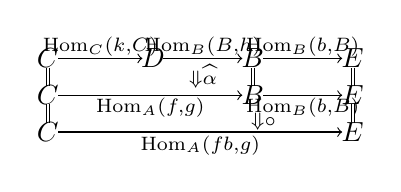
\begin{tikzpicture}[x=0.95em,y=0.95em]
  \node at (-4.6,2.3) {$C$};
  \node at (-0.6,2.3) {$D$};
  \node at (3.2,2.3) {$B$};
  \node at (7.0,2.3) {$E$};
  \draw[->] (-4.2,2.3) -- (-1.0,2.3);
  \node at (-2.6,2.75) {$\scriptstyle\HomC(k,C)$};
  \draw[->] (-0.2,2.3) -- (2.8,2.3);
  \node at (1.3,2.75) {$\scriptstyle\HomB(B,h)$};
  \draw[->] (3.6,2.3) -- (6.6,2.3);
  \node at (5.1,2.75) {$\scriptstyle\HomB(b,B)$};
  \draw[double,double distance=0.6pt] (-4.6,1.95) -- (-4.6,1.25);
  \draw[double,double distance=0.6pt] (3.2,1.95) -- (3.2,1.25);
  \draw[double,double distance=0.6pt] (7.0,1.95) -- (7.0,1.25);
  \node at (1.3,1.6) {$\scriptstyle\Downarrow\widehat{\alpha}$};
  \node at (-4.6,0.9) {$C$};
  \node at (3.2,0.9) {$B$};
  \node at (7.0,0.9) {$E$};
  \draw[->] (-4.2,0.9) -- (2.8,0.9);
  \node at (-0.7,0.42) {$\scriptstyle\HomA(f,g)$};
  \draw[->] (3.6,0.9) -- (6.6,0.9);
  \node at (5.1,0.42) {$\scriptstyle\HomB(b,B)$};
  \draw[double,double distance=0.6pt] (-4.6,0.55) -- (-4.6,-0.15);
  \draw[double,double distance=0.6pt] (7.0,0.55) -- (7.0,-0.15);
  \node at (3.6,-0.1) {$\scriptstyle\Downarrow\circ$};
  \node at (-4.6,-0.5) {$C$};
  \node at (7.0,-0.5) {$E$};
  \draw[->] (-4.2,-0.5) -- (6.6,-0.5);
  \node at (1.2,-1.0) {$\scriptstyle\HomA(fb,g)$};
\end{tikzpicture}
\end{center}
名为 $\circ$ 的两个\trCanonical{}\trCell{}都是复合；由 $\alpha$ 的正合性，$\widehat{\alpha}$ 也是复合，于是由引理 8.3.3 或引理 8.3.8，该粘贴胞腔亦是复合。由 $\beta$ 的正合性，$\widehat{\beta}$ 亦为复合；并再次由引理 8.3.3 或引理 8.3.8 得 $\widehat{\alpha q\cdot f\beta}$ 为复合，这就证明了矩形
$\alpha q\cdot f\beta\colon g(kq)\Rightarrow(fb)p$ 的正合性。
\end{proof}

\subsection*{练习}

\begin{exercise}\label{ex:exact-square-up-to-isomorphism}
对任何\trExactSquare
\begin{center}
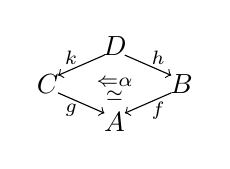
\begin{tikzpicture}[x=1.05em,y=1.05em]
  \node at (0,2.6) {$D$};
  \node at (-2.3,1.3) {$C$};
  \node at (2.3,1.3) {$B$};
  \node at (0,0) {$A$};
  \draw[->] (-0.35,2.3) -- (-1.95,1.6);
  \node at (-1.5,2.2) {$\scriptstyle k$};
  \draw[->] (0.35,2.3) -- (1.95,1.6);
  \node at (1.5,2.2) {$\scriptstyle h$};
  \draw[->] (-1.95,1.0) -- (-0.35,0.3);
  \node at (-1.5,0.4) {$\scriptstyle g$};
  \draw[->] (1.95,1.0) -- (0.35,0.3);
  \node at (1.5,0.4) {$\scriptstyle f$};
  \node at (0,1.35) {$\scriptstyle\Leftarrow\alpha$};
  \node at (0,0.9) {$\scriptstyle\simeq$};
\end{tikzpicture}
\end{center}
证明：将此方块与任何一组\trIsomorphism{} $\beta\colon f'\cong f$、
$\gamma\colon g\cong g'$、$\delta\colon h'\cong h$ 与 $\epsilon\colon k\cong k'$ 复合所得的方块也是正合的。
\end{exercise}

\begin{exercise}\label{ex:prove-trivial-exact-squares}
证明\cref{lem:trivial-exact-squares}。
\end{exercise}
